\documentclass[11pt,a4paper]{article}
\pdfinfoomitdate=1\pdftrailerid{}
\usepackage[margin=25mm]{geometry}
\usepackage{amsmath,amssymb,booktabs,array,graphicx,hyperref,xurl,float}
\hypersetup{hidelinks}\setlength{\parindent}{0pt}\setlength{\parskip}{6pt}
\newcolumntype{P}[1]{>{\raggedright\arraybackslash}p{#1}}
\renewcommand{\thesection}{S\arabic{section}}
\renewcommand{\thetable}{S\arabic{table}}
\renewcommand{\thefigure}{S\arabic{figure}}
\title{Supplementary technical notes for WorkCert}
\author{Saisai Hou \and Yunzhi Zhu \and Sen Zhang}
\date{SoftwareX manuscript SOFTX-D-26-01576\\Revision 1}
\begin{document}\maketitle
These notes describe the additional protocols, numerical checks and usage policies accompanying the revised article. Supplementary S2 contains their executable scripts, case-level results and manuscript build inputs. The released WorkCert runtime remains version 0.3.0. Original source files and original numerical results are preserved; the revision adds a separate \path{revision_r1} directory.

\section{Contribution and reconstruction measures}
A force--displacement table can be simplified and integrated with established numerical tools. WorkCert organizes additional information needed when the dense reference is held by a producer and only the reduced table is passed to a consumer. Table~\ref{tab:features} compares these workflows; it is a comparison of responsibilities, rather than a claim that existing libraries cannot be combined to implement them.

\begin{table}[H]\small\centering
\caption{Tasks in a table-exchange workflow.}\label{tab:features}
\begin{tabular}{P{.22\linewidth}P{.31\linewidth}P{.37\linewidth}}\toprule
Task&Simplifier and integrator workflow&WorkCert interface\\\midrule
Select nodes&Use geometric or fitting criteria&Built-in selectors or import external source indices\\
Evaluate work&Integrate the chosen interpolant&Reusable prefix and interval queries with cached local sums\\
Track source-relative error&Evaluate and retain the reference residual separately&Continuous residual extrema and area measures stored with the table\\
Exchange and check&Define a file format, units and verification rules&Versioned JSON, native-unit labels, source fingerprint and payload checksum\\
Refine a decision&Carry interval budgets between producer and consumer&Consumer queries share the stored error policy; examples request only unresolved records\\
Accept a cyclic path&Carry status and branch direction through aggregation&S2's application wrapper rejects unmet or unknown local budgets before qualified use\\\bottomrule
\end{tabular}\end{table}

For $r=F-\widehat F$ and $D(u)=\int_0^u r(s)\,ds$, terminal error $d=D(U)$ is signed; $\eta=\int|r|$, $\xi=(\eta+|d|)/2$, $E_p=\max|D|$, $E_w=\max D-\min D$, and $\delta=\max|r|$. Work quantities use force times displacement; $\delta$ uses force. Prefix errors include the initial value $D(0)=0$. Extrema of the piecewise-quadratic primitive occur at source nodes or residual zeros within source segments.

For any $a\leq b$, $\int_a^b r=D(b)-D(a)$. The interval joining the minimum and maximum of $D$, in either order, attains the range in absolute value. Hence $E_w$ is the discrepancy norm described by Bouchot and Bauer (2014), DOI \url{https://doi.org/10.1016/j.cam.2014.05.012}. This established norm is part of WorkCert's mathematical background.

A vertical error limit implies $|\int_a^b r|\leq\delta(b-a)$ but does not account for the actual residual sign pattern. Conversely, a small signed terminal error can conceal larger intermediate errors. WorkCert therefore records several measures so users can select the one matching their query. Neither a new norm nor a universally optimal selector is claimed. The quantities concern the supplied numerical reference; they do not include measurement uncertainty or enclose floating-point rounding.

\section{Selection and stopping protocols}
Work priority initializes the endpoints and the requested force peak. Each active chord $(a,b)$ has score $\eta_{ab}$ and split index $j=\arg\max_{a<i<b}|r_i|$. The heap key is $(-\eta_{ab},a,b)$: ties select the smallest left endpoint, then right endpoint. The first maximizing interior source index is inserted; the parent is replaced by $(a,j)$ and $(j,b)$. The split maximizes vertical deviation, not the decrease in area. Vertical priority replaces the score by $\delta_{ab}$. Summaries are recombined along the balanced tree; errors are reevaluated after every insertion because refinement errors need not be monotone.

The fixed-count RDP baseline in \path{validation/baselines.py} uses
\[
x_i'=(x_i-x_0)/(x_{n-1}-x_0),\qquad
F_i'=(F_i-\min F)/(\max F-\min F).
\]
A zero force range is replaced by one. Perpendicular distance to the normalized endpoint chord chooses each split, and best-first refinement chooses the chord with greatest distance. Endpoints and the first absolute force maximum are protected before refinement. Every protected point counts toward $K$. Errors are evaluated in the original units. The separate epsilon-based, unanchored RDP routine is used for agreement checks with third-party implementations; it is not substituted for fixed-count RDP in the main comparison.

The stopping audit covers 70 original references: 23 CX-steel records, one enhanced double-arrow honeycomb (EDAH) record, and 46 PLA+ records. Two selectors and four stopping measures give 560 cases. Each case uses the full source length as its cap, endpoint and first-absolute-peak anchors, and tolerance $0.01|W(U)|$; all terminal reference works are nonzero. All cases meet tolerance. None are missing, excluded for failure, or stopped at the point cap. An independent scalar audit checks 3360 numerical fields, with maximum relative difference $2.70\times10^{-16}$.

Within work priority, stopping on $\eta$ retains median 27 nodes (range 9--51), whereas stopping on $E_w$ retains median 14 (range 6--27). Both satisfy the same all-interval requirement. The prefix-only median of 12.5 addresses a different query domain. For vertical priority, the corresponding $\eta/E_w$ medians are 28/15. These values compare stopping measures within a selector, rather than comparing different selection algorithms.

Exact fixed-vertex controls use the 58 unaltered references with $n\leq1000$ (12 CX and 46 PLA+). Eleven longer CX records and EDAH are excluded by length, without downsampling. The threshold is a computational budget for the benchmark: edge preparation scans all source cells of all candidate edges, requiring $O(n^3)$ work; the subsequent dynamic program costs $O(Kn^2)$ with $O(n^2+Kn)$ storage. The two float64 edge matrices alone occupy 16,000,000 bytes at $n=1000$. Five budgets and two objectives give 580 solutions. The optimized objectives are $\eta$ and $\delta$, under the same endpoint and peak constraints; prefix and window optimality is not inferred.

\section{Workbook acceptance and endpoint reconciliation}
The original 45/46 result tests whether workbook EA, SEA, MCF and CFE values lie within the reduced-table intervals at the reported stroke. A numerical slack of $10^{-9}$ in each metric's native unit is allowed at either endpoint. Peak force covers 46/46. This is interval containment, not equality of point estimates and not an experimental-repeatability test.

Specimen 05 is the sole interval-coverage exception. Its published EA exceeds the reference integral to nominal 50 mm by 0.0647365134 J. Thirteen nominal-50-mm records were integrated in the workbook to stored endpoints between 50.004 and 50.009 mm. For these thirteen only, the aligned audit integrates through that endpoint. The remaining 33 retain their reported cutoff: some original records extend substantially farther, so using every record's final sample would be incorrect.

The independent audit reads the original XLSX values, performs exact rational arithmetic on their binary floating-point values, and rounds each final metric once. SEA uses the reported mass. MCF retains the workbook's reported stroke denominator even for the thirteen small overshoots; CFE uses MCF divided by the appropriate prefix peak. Early-prefix peak intervals are retained rather than replacing them by a later global peak. The original comparison remains unchanged alongside the aligned results.

\begin{table}[H]\centering
\caption{Remaining differences after reproducing workbook endpoint conventions. Relative differences use the absolute published value.}
\begin{tabular}{lrrr}\toprule
Metric&Maximum absolute difference&Maximum relative difference&Coverage\\\midrule
EA (J)&$2.726\times10^{-10}$&$5.714\times10^{-13}$&46/46\\
SEA (kJ/kg)&$9.667\times10^{-12}$&$5.715\times10^{-13}$&46/46\\
MCF (kN)&$5.793\times10^{-12}$&$5.714\times10^{-13}$&46/46\\
PCF (kN)&0&0&46/46\\
CFE&$3.664\times10^{-13}$&$5.714\times10^{-13}$&46/46\\\bottomrule
\end{tabular}\end{table}

The two triplicate control groups provide descriptive scatter only. For a control mean, the interval endpoints are the means of the three specimen endpoints, without dividing the reconstruction bound by $\sqrt3$. At 10 mm, nominal SCMC has bound/SD ratio 0.921; three repeats do not provide a precise population SD. The $\pm0.05$ g scenario represents rounding to 0.1 g, not a measured mass uncertainty. Its maximum SEA change is 0.310\%. For configurations 26 and 35, rounding makes the full-reference worst-case difference $-0.00344798$ kJ/kg, so further curve refinement cannot settle that comparison.

\section{Checked cyclic composition and recovery}
The original WorkCert API returns error metadata even when a point cap prevents tolerance attainment. It does not automatically disable later queries. The new \path{revision_r1/checked_cyclic_path.py} is an application wrapper with explicit acceptance semantics. It requires every branch's stored flag to be true and its reported measure to satisfy the recorded budget. It checks units, source-edge coverage and summary consistency, propagates failed IDs, and raises \path{PathToleranceError} by default. Diagnostic mode returns \path{valid_for_downstream_use=False}; this report must not be treated as budget-qualified input.

No failed branch may be dropped. A zero-displacement event retains chronological coverage and contributes zero work. Branch records must come from source-verified tables; a checksum detects payload inconsistency but does not authenticate a producer. Unit labels are checked for agreement and do not convert values. An absent or unknown tolerance is not treated as a passing result.

The recovery calculation hash-checks and verifies all 2971 original tables against their source. Only branch 2533 fails its local budget. Raising its cap from 129 to 257 produces 153 retained points out of 1663 source points and meets the unchanged budget. Other branches and all 1984 dwell events are retained unchanged. If refinement is unavailable or still insufficient, retain and verify the full branch or continue to reject the path for the requested use. Never silently increase its allowed error.

\begin{table}[H]\centering
\caption{Targeted recovery without relaxing the branch budget.}
\begin{tabular}{lrr}\toprule
Quantity&Initial&Recovered\\\midrule
Branch 2533 retained nodes&129&153\\
Branch window error (J)&0.1542233705&0.0820252318\\
Branch requested budget (J)&0.0871937363&0.0871937363\\
Total branch nodes&13,890&13,914\\
Failed branches&1&0\\
Signed terminal error (J)&68.529837535&68.488116925\\
Chronological prefix error (J)&68.720971127&68.679250517\\
Chronological window error (J)&68.945668396&68.903947786\\
Sum of branch window bounds (J)&104.48&104.405590720\\\bottomrule
\end{tabular}\end{table}

The accepted-path flag establishes the prescribed local branch budgets only. A separately specified global path budget must be tested against the composed prefix/window error. For descending traversal, a branch summary transforms to $(-d,l-d,h-d)$ before chronological concatenation. This is a real-arithmetic identity evaluated with sequential float64 operations; it does not enclose rounding. For example, the sequence $[10^{16},1,-10^{16}]$ sums sequentially to zero rather than one. The recovered example's independent compensated scalar integration differs from the composed extrema by at most $7.11\times10^{-14}$ J. Twenty-five policy and composition tests accompany the script.

The reference's 92.034 kJ is signed path work. A closed quasi-static cycle returning to the same stored-energy state has a loop integral associated with hysteretic dissipation; orientation determines its sign. An open record can also change stored energy. This record begins at $(0\ \mathrm{mm},0\ \mathrm{kN})$ and ends at $(3.1154\ \mathrm{mm},13.0479\ \mathrm{kN})$. Its chronological net work must therefore not be labeled total closed-cycle dissipation. The 94-reversal diagnostic is separate from branch splitting and is consistent with the 47-cycle S1-L1 entry in Table 3 of the cited source paper.

\section{Serialized sizes and timing protocol}
The exchange experiment uses all 70 references and fixes work-priority tables at 33 nodes with endpoints and the absolute peak. It writes real compact JSON files in three forms: the complete reduced WorkCert schema; a full-node table in that same schema; and minimal dense JSON containing coordinates, force, units and a reference hash. The latter omits retained indices, error metadata, payload checksum and integration caches. Sizes are measured as file bytes before archive compression.

Across curves, median sizes are 1712.5, 20,401 and 16,027.5 bytes, respectively. The median contribution of the reduced table's fixed fields with empty arrays is 1066 bytes. Thus metadata is a substantial part of the small exchanged file and is included in every reported size.

Measurements use three newly launched sequential Python processes, one warm-up and five timed repetitions per load/query operation in each process. Locations are deterministic (seed 20261123): 10,000 uniform prefixes and 10,000 windows formed from sorted pairs of uniform positions. The per-process median is combined into a per-curve median across processes; the article then reports the median across curves. The plotted interquartile ranges describe differences among curves, not confidence intervals or repeat timing noise. Individual measurements and per-curve values are retained in S2.

The environment is Windows 10, Intel Core i5-11300H @ 3.10 GHz, 8 logical processors, 15.6867 GiB physical memory available to the operating system, Python 3.12.14 and NumPy 2.3.5. Files use a warm operating-system cache. WorkCert load timing includes UTF-8 input, JSON parsing, schema/checksum/invariant checks and cache construction. Minimal dense loading only parses coordinates into arrays, so its 0.589 ms median is a weaker operation than reduced/full-schema loads of 0.758/3.101 ms. The experiment does not claim universal loading acceleration.

For 10,000-query batches, reduced/full-schema prefix medians are 2.832/5.106 ms and window medians are 3.427/5.976 ms. An untimed observer applies the exact runtime fallback predicate and delegates to the unchanged method. No fallback occurs among 1.4 million tested locations for either representation. A separately reported 100,001-node positive-force example broadens the input-size range; all case-level results remain available rather than being pooled into the 70 experimental records.

The cancellation stress fixture uses 33, 1001 and 100,001 retained nodes and 256 full-domain window queries. Each of three processes records three timed repetitions after warm-up. At the largest size, the actual runtime takes 2.278 s and returns $2\times10^{-100}$ J, while a diagnostic bypass takes 0.900 ms and returns zero. The bypass is an ablation, not an alternate supported mode. It exposes the cost of the direct-summation safeguard; ordinary-record counts and stress-test timings are reported separately. Four diagnostic tests check the serialized representations and observer/bypass logic.

\section{Precision and original construction controls}
A 100,001-point constant reference, $x_i=10^{-4}i$ mm and $F_i=0.1$ kN, reduces to two endpoints with zero reconstruction error and 1 J terminal work. Constant/affine tests vary length and coordinate/force scales. At one million intervals, computed source work differs from the correctly rounded exact binary-input integral by one ULP (Fig.~\ref{fig:precision}).

For $x=[0,1,2]$ and $F=[10^{16},0,1]$, full retention gives $E_w=0$, while subtraction of rounded global prefixes loses the 0.5 J window $[1,2]$. Direct local integration returns 0.5 J. A signed unit-step record $F=[0,10^{16},1,-10^{16},0]$ returns 1 J when both components of each endpoint mean are retained. A $10^{12}$-baseline example has $E_p=0.010009765625$ J; replacing its metadata by zero is rejected. These fixtures separate representation error from arithmetic behavior.

\begin{figure}[H]\centering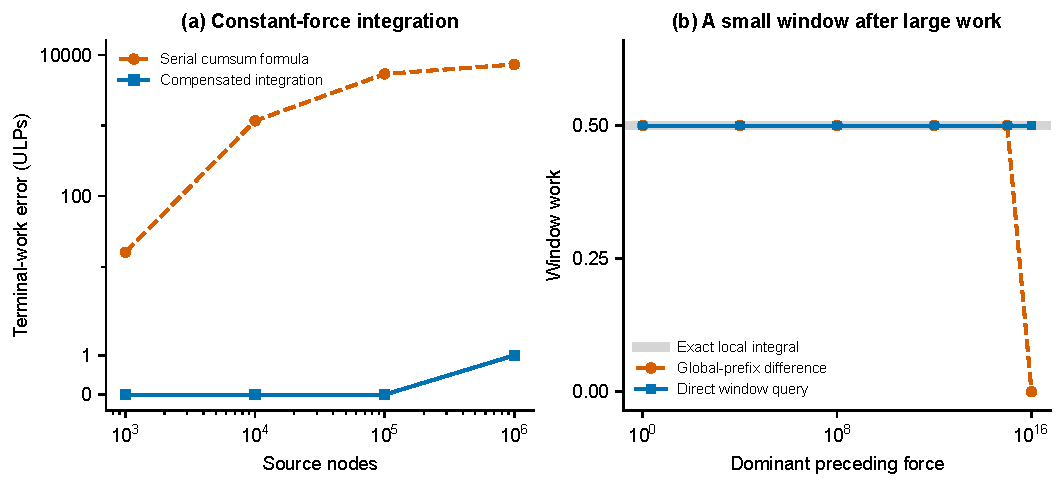
\includegraphics[width=\linewidth]{figures/fig01_numerics.pdf}
\caption{Original arithmetic fixtures: terminal-work error against exact binary-input integration and local-window integration after a dominant preceding force. OpenAI Codex assisted with the archived plotting code.}\label{fig:precision}\end{figure}

The original construction benchmark uses $10^3$--$10^6$ synthetic points and three relative tolerances, with three independent paired processes on the recorded host. At one million points and 0.1\% window tolerance, full-scan version 0.1 takes median 11.78 s and the stable incremental implementation takes 4.88 s, with 107 retained nodes. Complete error evaluations decrease from 105 to one. The small-input overhead and all timing replicates are retained (Fig.~\ref{fig:originalscale}). New exchange timings are separate measurements rather than replacements for this original experiment.

\begin{figure}[H]\centering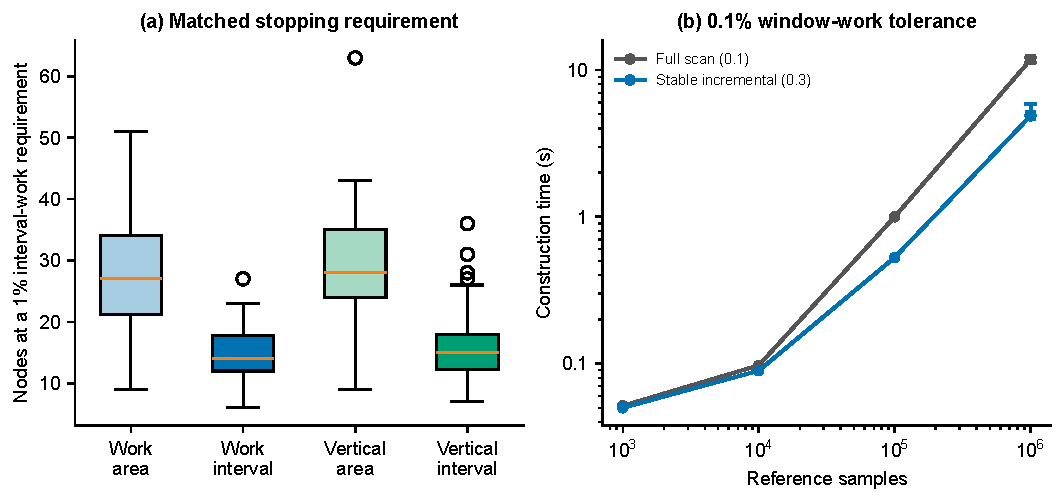
\includegraphics[width=\linewidth]{figures/fig05_scaling.pdf}
\caption{Original within-selector stopping and construction measurements. Boxes give quartiles and medians with 1.5-interquartile-range whiskers; timing ranges use three independent paired processes. OpenAI Codex assisted with the archived plotting code.}\label{fig:originalscale}\end{figure}

\section{Reproduction files and provenance}
The full original input snapshot is \url{https://github.com/changs1723/WorkCert/tree/article-v0.3.0-final}; the runtime is \url{https://doi.org/10.5281/zenodo.23934502}. Supplementary S2 overlays a separate \path{revision_r1} directory onto that fixed source root. Its README provides installation, verification, recomputation and article-building commands. The original source manifest and a separate revision manifest distinguish existing inputs from new files. The software version and the article revision are separate identifiers.

Key entry points are \path{audit_protocols.py}, \path{recompute_cyclic_recovery.py}, \path{benchmark_exchange.py}, \path{build_revision_figures.py} and \path{build_revision.py}, all under \path{revision_r1}. Saved outputs include all 560 stopping cases, 230 workbook metric rows, branch-acceptance records, 70 per-curve exchange records and individual timings. Verification operates in an isolated copy when a component writes reports. Timing reproduction is optional because its values depend on host load; the archived protocol and raw repetitions permit inspection independently of rerunning it.

The original released package has 81 test methods (759 check records). Both wheel and source distributions passed six Windows installations; the version-tag workflow passed all 15 jobs across Linux, macOS and Windows with Python 3.10--3.14. These historical results are retained in the fixed source's \path{release_evidence} directory. The revision separately adds 25 acceptance-wrapper tests, four exchange-diagnostic tests, a 560-case stopping audit, a 230-row workbook audit, and full cyclic recovery verification. The original contributor-verification record is retained at its original date. The revision scripts and tests were developed and executed with Codex assistance; their inputs, environments and verification results are recorded in the accompanying files.

\section*{Declaration of generative AI and AI-assisted technologies in the manuscript preparation process}
OpenAI Codex (OpenAI) assisted with research planning, literature and public-data collection, implementation and debugging, numerical analysis and verification, figure preparation, drafting, language editing and typesetting. The authors are responsible for the research design, interpretation, software, results and final manuscript.
\end{document}
